\renewenvironment{longtable}{\rowcolors{2}{LightGray}{white}\oldlongtable} {\endoldlongtable}
\chapter{GPIO操作及其中断}
\section{GPIO简介}
\ac{GPIO}是指通用目的输入输出设备。在STM32上,它以几组引脚的形式引出,可以连接其他电路组件,例如LED灯,此外,许多引脚有特定的复用功能,例如可以作为串口通信的Rx和Tx引脚,连接串口设备,例如GPS等。GPIO是STM32上最基本的外设,因此在这里我们首先来学习GPIO的一些基本应用,以此引出操作STM32外设的一般编程流程。
\par 
STM32的GPIO是一个比较高级的IO外设,不同于,每个引脚都支持几种不同的模式,适用于不同的应用场景,有的引脚还支持高达5V的输入电压。GPIO的基本电路结构如下图\footnote{截自\acs{RM}}。
\par 
\begin{figure}[h]
	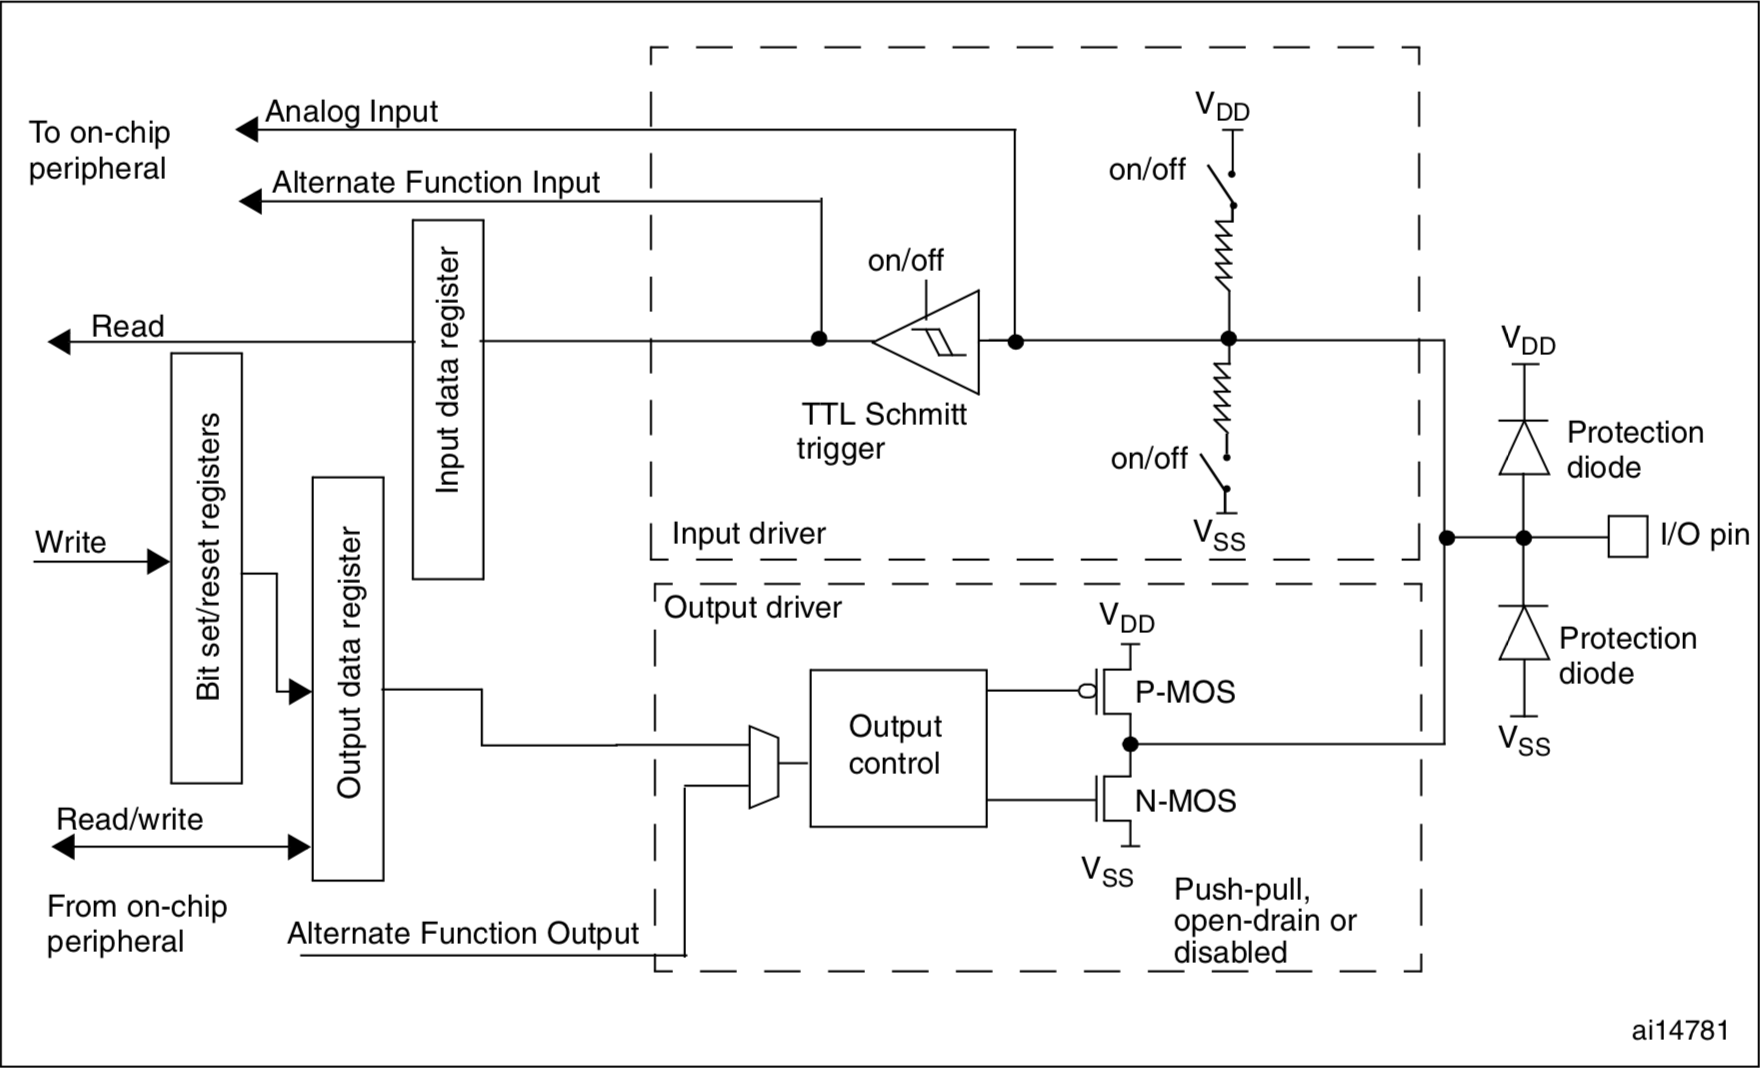
\includegraphics[width=\textwidth]{images/content/gpioCircuit.png}
	\captionof{figure}{GPIO基本结构}
	\label{fig:gpioCircuit}
\end{figure}
\par 
\newpage
GPIO支持的模式见下表:
\begin{center}
	\begin{longtable}[l]{| p{30mm} | p{40mm} | p{70mm} |}
		\caption{GPIO模式}\\
		\hline 
		\rowcolor{Gray}
		\textbf{类型} & \textbf{模式名称} & \textbf{简要描述} \\
		\hline
		\endfirsthead
		
		\hline 
		\rowcolor{Gray}
		\textbf{类型} & \textbf{模式名称} & \textbf{简要描述} \\
		\hline
		\endhead
		
		输出模式 & 推挽输出  & 电流较大的输出模式 \\
		输出模式 & 漏极开路输出 & 可以双向通信的输出模式,一般用于模拟通信协议(例如IIC) \\
		输出模式 & 复用推挽输出 & 作为复用功能时的推挽输出模式 \\
		输出模式 & 复用漏极开路输出 & 作为复用功能时的开漏输出模式 \\
		输入模式 & 浮空输入  & 完全悬空的输入模式 \\
		输入模式 & 上拉输入  & 内部接入上拉电阻的输入模式 \\
		输入模式 & 下拉输入  & 内部接入下拉电阻的输入模式 \\
		输入模式 & 模拟输入  & 输入ADC时使用的模式 \\
		
		\hline
	\end{longtable}
\end{center}
\par 
在使用的时候,应当仔细分析应用场景,找出适合的模式。接下来,我们通过几个简单的例子,了解GPIO常用的操作以及对应的库函数用法。
\section{GPIO常用操作}
在STM32中,使用一个外设必须首先完成初始化操作,包括初始化对应的外设模块,打开对应的时钟信号,某些外设还要求产生软件启动指令才能正常工作。我们假设目前的场景下,单片机连接的外部元件如下表所示:
\begin{center}
	\begin{longtable}[l]{| p{20mm} | p{80mm} | p{40mm} |}
		\caption{单片机引脚定义}\\
		\hline 
		\rowcolor{Gray}
		\textbf{引脚} & \textbf{连接的元件} & \textbf{需要使用的模式} \\
		\hline
		\endfirsthead
		
		\hline 
		\rowcolor{Gray}
		\textbf{引脚} & \textbf{连接的元件} & \textbf{需要使用的模式} \\
		\hline
		\endhead
		
		PA0 & LED灯(另一侧通过限流电阻接3.3V)  & 推挽输出 \\
		PA1 & LED灯(另一侧通过限流电阻接3.3V)  & 推挽输出 \\
		PA2 & 按钮(另一侧接3.3V) & 下拉输入 \\
		PA3 & 按钮(另一侧接0V) & 上拉输入 \\
		
		\hline
	\end{longtable}
\end{center}
\par 
在这个例子当中,我们将依次完成LED闪烁、流水灯、按钮控制LED灯的实验。下面,让我们看一看具体的代码实现。
\par 
这个例子中,我们需要在工程文件夹下的User/文件夹下新建GPIO.c和GPIO.h两个文件,以模块的形式向外部提供接口。

	\subsection{预备工作}
	我们首先来填入GPIO.h这个头文件:
	\par 
	\begin{lstlisting}[language=bash, style=customStyleC, caption=GPIO.h]
#ifndef __GPIO_H__
#define __GPIO_H__

#include "stm32f10x.h" 
#include "stm32f10x_conf.h" 

void PinsInit();
void LED1Operation(u8 on);
void LED2Operation(u8 on);
u8 Button1Pressing();
u8 Button2Pressing();

#endif
	\end{lstlisting}
	\par 
	头文件中首先引入了两个外设库提供的头文件,利用这两个头文件就可以访问外设库中的全部函数。之后,我们声明了5个函数,第一个的功能是初始化用到的引脚,此后的两个函数操作对应的LED灯,最后两个函数用于检查两个按钮是否按下。这些函数的实现都放在GPIO.c文件中。要注意的是,在C语言中,并没有bool等布尔类型,因此我们需要使用u8代替,顾名思义,u8表示这个类型是无符号(unsigned)8位整型。在我们编写GPIO.c中的代码时,需要包含这个头文件。如果读者学习过C语言的模块化设计,应该很熟悉这种操作。
	\subsection{GPIO的初始化}
		下面这个函数完成用到的GPIO的初始化,位于GPIO.c文件中。
		\par 
		\begin{lstlisting}[language=bash, style=customStyleC, caption=GPIO初始化]
void PinsInit() {
	GPIO_InitTypeDef gpioInitStruct;
	
	RCC_APB2PeriphClockCmd(RCC_APB2Periph_GPIOA, ENABLE);
	
	gpioInitStruct.GPIO_Mode = GPIO_Mode_Out_PP;
	gpioInitStruct.GPIO_Pin = GPIO_Pin_0 | GPIO_Pin_1;
	gpioInitStruct.GPIO_Speed = GPIO_Speed_50MHz;
	GPIO_Init(GPIOA, &gpioInitStruct);
	
	gpioInitStruct.GPIO_Mode = GPIO_Mode_IPD;
	gpioInitStruct.GPIO_Pin = GPIO_Pin_2;
	GPIO_Init(GPIOA, &gpioInitStruct);
	
	gpioInitStruct.GPIO_Mode = GPIO_Mode_IPU;
	gpioInitStruct.GPIO_Pin = GPIO_Pin_3;
	GPIO_Init(GPIOA, &gpioInitStruct);
}
		\end{lstlisting}
		\par 
		函数的第2行定义了一个GPIO初始化结构体,以备之后使用。\\
		第4行调用库函数打开了GPIOA的时钟。读者应当注意到其中APB2Periph这个短语,这表示GPIOA这个外设是属于APB2时钟线上的外设。这个结论来自于Datasheet,如图\ref{fig:clockDiag}所示。
		\\
		第6~9行设置PA0和PA1的模式为推挽输出(Push-Pull output)模式,最大输出频率为50MHz。
		\begin{figure}[htbp]
			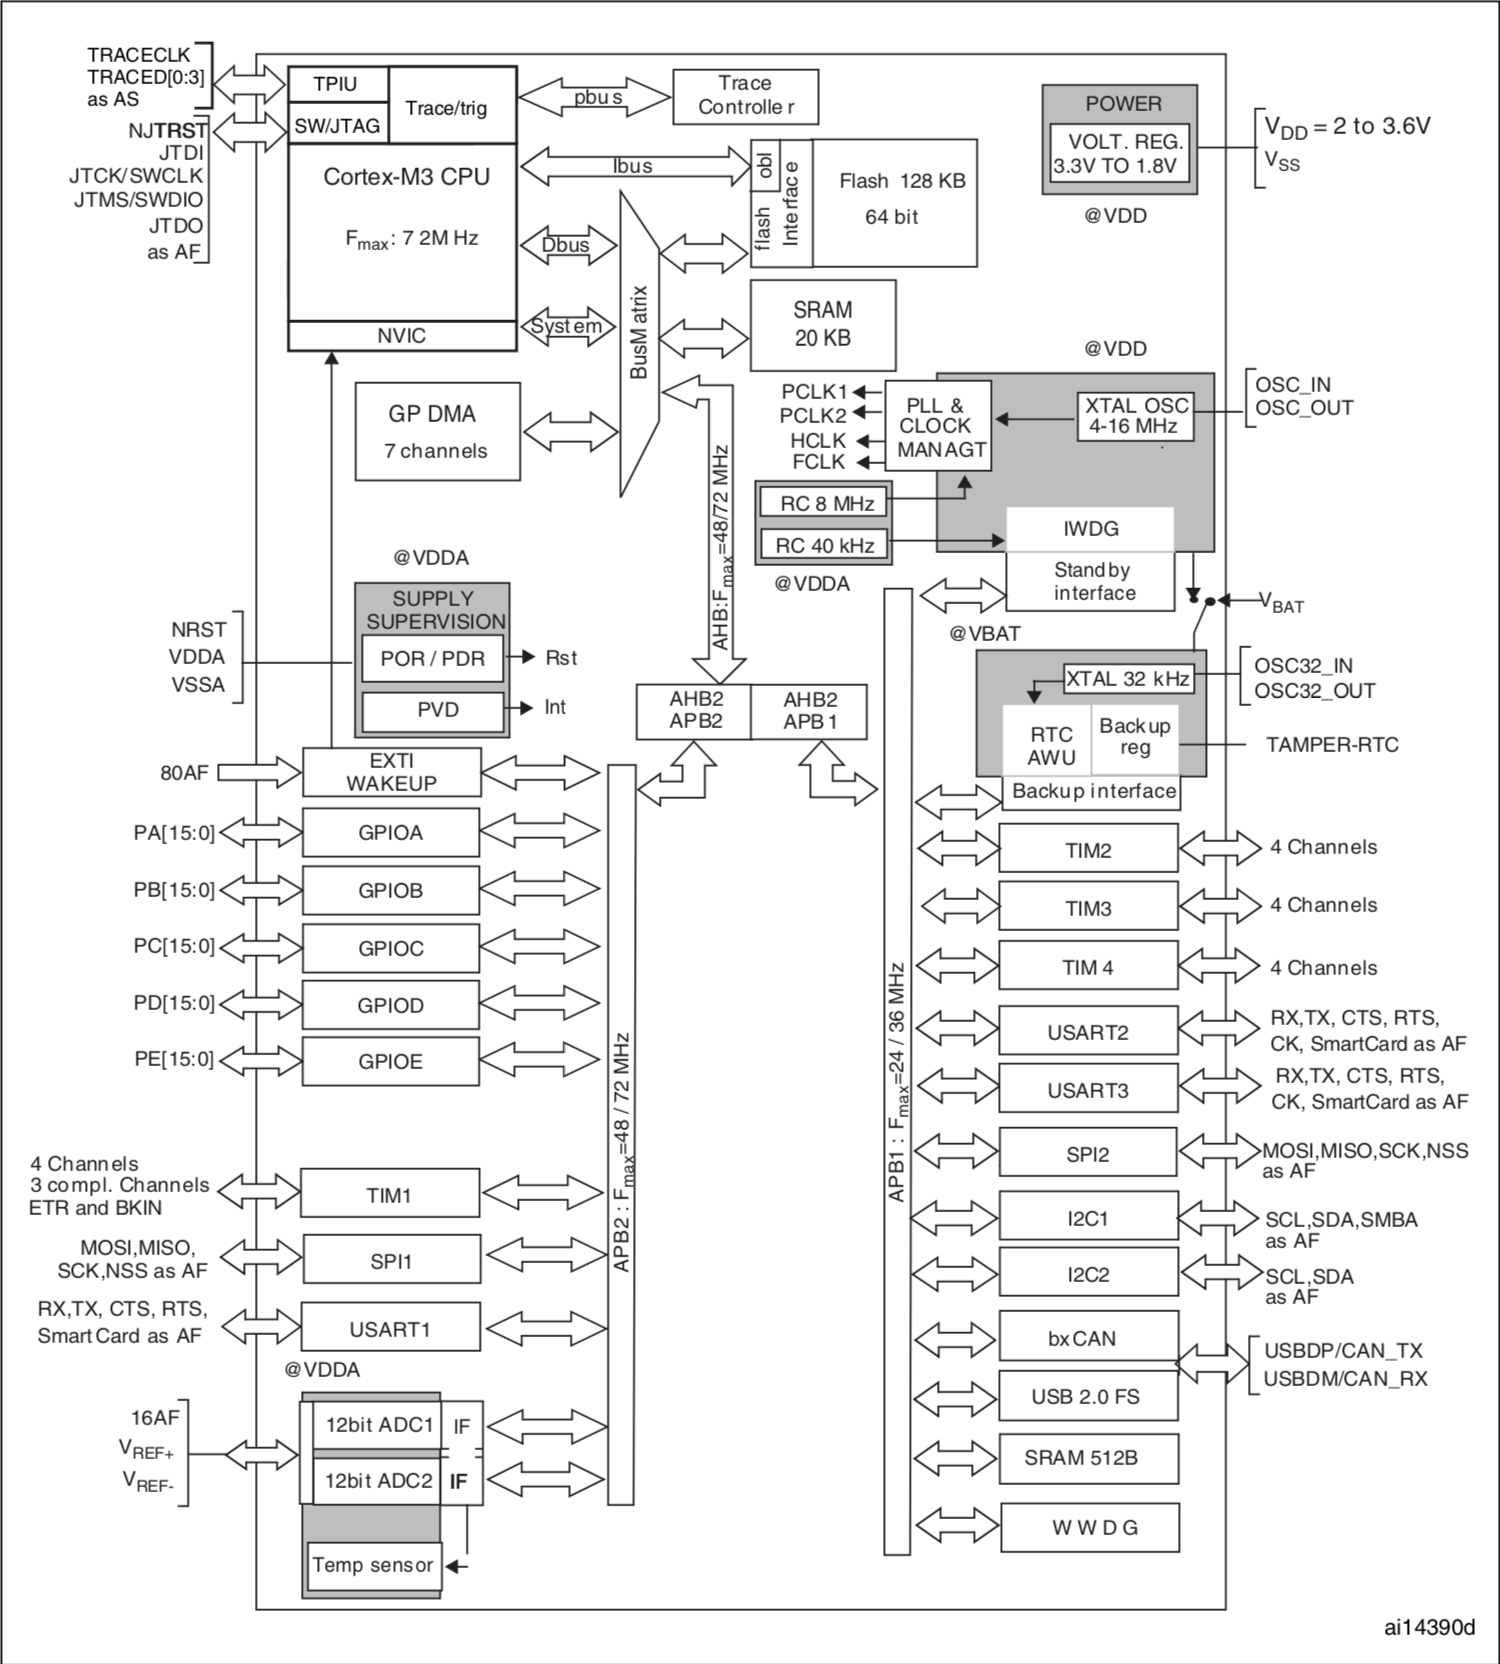
\includegraphics[width=\textwidth]{images/content/clockDiag.png}
			\captionof{figure}{STM32时钟线}
			\label{fig:clockDiag}
		\end{figure}
		
		


















